% TODO add tech / software table?
\section{Materials and methods}
In this section I will describe the development of the interactive visualization
as well as the process of gathering information on how people use it.

\subsection{Helsinki region Travel Time Matrix}

The \acrlong{ttm} (referred to as \acrshort{ttm} from here onwards)
is a dataset containing information of travel times and distances
in the Helsinki region in southern Finland.
This dataset is crucial to developing the map application,
as it is the sole source of the travel times shown on the map.

% Describe ttm in general: ykr, origin dest pairs etc (more surface level stuff common to all matrices)
A significant component of the \acrshort{ttm} is the \acrlong{ykr} (\acrshort{ykr}) grid
made by Statistics Finland.
The grid has a spatial resolution of 250x250m, and it covers the entire Finland.
Most importantly, however, the part of the \acrshort{ykr} grid that overlaps with
the Helsinki region provides the spatial component for
the travel times stored in the \acrshort{ttm}.
The basic idea of the \acrshort{ttm} is that it stores the travel times and distances
from every \acrshort{ykr} grid cell to every grid cell within the Helsinki region.
The Helsinki region fits 13231 \acrshort{ykr} grid cells,
which means that the complete \acrshort{ttm} contains travel times and distances for
over 175 million routes.

All the routes are calculated for multiple different travel modes.
The primary travel modes are walking, cycling, public transportation and private car,
but, when applicable, each mode can have variations based on
time of day and / or walking or cycling speed.
Time of day is especially relevant to motorized transport
in the form of the rush hour, for example,
while walking speed affects any travel mode
where a significant portion of the trip is covered on foot.

% TODO talk briefly about methodology, open source

% Describe the particular matrix (2023), methodology etc
There are matrices from many years.
This visualization is based on the 2023 version of the \acrshort{ttm}
\parencite{fin2023}.
The version of the \acrshort{ttm} used in this visualization is at the time of writing the newest one

\begin{table}[H]
	\caption{Descriptive values of the \acrshort{ttm} \parencite{fin2023}}
	\label{tab:ttm indicators}
	\centering
	\begin{tabular}{ | L{0.4\textwidth} | L{0.5\textwidth} | }
		\hline
		Spatial resolution
		& 250 x 250 m
		\\
		\hline
		Number of grid cells
		& 13231
		\\
		\hline
		Number of origin-destination pairs
		& 175 059 361
		\\
		\hline
		Travel modes
		& \tabitem walking \\
		& \tabitem cycling \\
		& \tabitem public transportation \\
		& \tabitem private car \\
		\hline
		Travel mode variations (if applicable)
		& \tabitem Time of day (rush hour, midday, night) \\
		& \tabitem Walking speed (average, slow) \\
		& \tabitem Cycling speed (average, fast, slow) \\
		\hline
	\end{tabular}
\end{table}

\begin{table}[H]
	\caption{The table structure of \acrshort{ttm} data \parencite{fin2023}}
	\label{tab:ttm table structure}
	\centering
	\begin{tabular}{ | L{0.15\textwidth} | L{0.75\textwidth} | }
		\hline
		Column name
		& Description
		\\
		\hline
		\hline
		from\_id
		& ID number of the origin grid cell
		\\
		\hline
		to\_id
		& ID number of the destination grid cell
		\\
		\hline
		walk\_avg
		& Travel time in minutes from origin to destination by walking at an average speed
		\\
		\hline
		walk\_slo
		& Travel time in minutes from origin to destination by walking slowly
		\\
		\hline
		bike\_avg
		& Travel time in minutes from origin to destination by cycling at an average speed; incl. extra time (1 min) to unlock and lock bicycle
		\\
		\hline
		bike\_fst
		& Travel time in minutes from origin to destination by cycling fast; incl. extra time (1 min) to unlock and lock bicycle
		\\
		\hline
		bike\_slo
		& Travel time in minutes from origin to destination by cycling slowly; incl. extra time (1 min) to unlock and lock bicycle
		\\
		\hline
		pt\_r\_avg
		& Travel time in minutes from origin to destination by public transportation in rush hour traffic, walking at an average speed
		\\
		\hline
		pt\_r\_slo
		& Travel time in minutes from origin to destination by public transportation in rush hour traffic, walking at a slower speed
		\\
		\hline
		pt\_m\_avg
		& Travel time in minutes from origin to destination by public transportation in midday traffic, walking at an average speed
		\\
		\hline
		pt\_m\_slo
		& Travel time in minutes from origin to destination by public transportation in midday traffic, walking at a slower speed
		\\
		\hline
		pt\_n\_avg
		& Travel time in minutes from origin to destination by public transportation in nighttime traffic, walking at an average speed
		\\
		\hline
		pt\_n\_slo
		& Travel time in minutes from origin to destination by public transportation in nighttime traffic, walking at a lower speed
		\\
		\hline
		car\_r
		& Travel time in minutes from origin to destination by private car in rush hour traffic
		\\
		\hline
		car\_m
		& Travel time in minutes from origin to destination by private car in midday traffic
		\\
		\hline
		car\_n
		& Travel time in minutes from origin to destination by private car in nighttime traffic
		\\
		\hline
		walk\_d
		& Distance from origin to destination, in metres, on foot
		\\
		\hline
	\end{tabular}
\end{table}

\subsection{Requirements for the interactive map presentation}
% What interaction should there be in the map
% What requirements do the two above chapters place on the map

% Why this must be considered
As mentioned earlier, cartographic visualization is often about tradeoffs.
The interactive map crafted here is no exception.
In addition to visual composition,  % TODO
many decisions must be made based on more technical basis.
For example, the sheer scale and detail of the dataset being visualized
means that instantaneous interaction with the map is not realistic
if no detail of the mapped data is to be sacrificed.
These kinds of tradeoffs are important to recognize,
because only through them is it possible to specify what
requirements should, or even could, be placed on the map application.

% Roughly what kind of a map? Why?
Based on the background study,  % TODO
I made the decision to prioritize real-time interaction over minute detail in the map.
The goal of the map is to act as a dynamic overview to the entire travel time matrix,
and user interaction, whether it is changing the location or travel mode,
should result in instant visual feedback on the map.
This decision is what ultimately shapes the requirements for the mapped data,
and thus dictates what kind of processing should be done on the data.

% TODO copypasta
Functional requirements define what a product must do,
what its features and functions are.
Nonfunctional requirements describe the general properties of a system.
Nonfunctional requirements can be further dividied into quality attributes
(how the software should be) and constraints (technical limitations)

\begin{table}[H]
	\caption{The functional requirements of the map application}
	\label{tab:functional requirements}
	\centering
	\begin{tabular}{ | L{0.3\textwidth} | L{0.6\textwidth} | }
		\hline
		Requirement
		& Description
		\\
		\hline
		\hline
		Location selection by clicking
		& The user can click on a location and produce an accessibility map of that location
		\\
		\hline
		Location selection by hovering
		& The user can hover their mouse over the map,
		and the map shows the accessibility of the location that is under the cursor,
		updating constantly as the cursor moves
		\\
		\hline
		Toggling between modes of location selection
		& The user can toggle their mode of interaction by clicking:
		Clicking while hovering locks the map, clicking while the map is locked resumes hovering
		\\
		\hline
		Interactive selection of travel mode
		& The user can choose the travel mode for which the travel times shown on the map are calculated
		\\
		\hline
	\end{tabular}
\end{table}

\begin{table}[H]
	\caption{Nonfunctional requirements}
	\label{tab:nonfunctional requirements}
	\begin{subtable}[h]{\textwidth}
		\caption{Quality requirements}
		\label{tab:quality requirements}
		\centering
		\begin{tabular}{ | L{0.2\textwidth} | L{0.7\textwidth} | }
			\hline
			Category
			& Requirements
			\\
			\hline
			\hline
			Performance
			& \tabitem Data serving speed allows for real-time interaction \\
			& \tabitem Map rendering speed allows for real-time interaction \\
			\hline
			Maintainability
			& \tabitem All components are as independent as possible \\
			& \tabitem The codebase is versioned and documented \\
			& \tabitem Deploying the application is reproducible \\
			\hline
			Usability
			& \tabitem Using the map is intuitive \\
			& \tabitem Visual feedback from user interaction is instantaneous \\
			\hline
			Scalability
			& \tabitem The application is scalable to meet different usage loads \\
			& \tabitem Different application components can be scaled independently \\
			\hline
		\end{tabular}
	\end{subtable}
	\newline
	\newline  % https://tex.stackexchange.com/questions/38893/cant-generate-vertical-space-between-tables
	\newline
	\begin{subtable}[h]{\textwidth}
		\caption{The constraints of the application}
		\label{tab:constraints}
		\centering
		\begin{tabular}{ | L{0.2\textwidth} | L{0.7\textwidth} | }
			\hline
			Constraint
			& Description
			\\
			\hline
			\hline
			Platform
			& The application runs in a web browser
			\\
			\hline
		\end{tabular}
	\end{subtable}
\end{table}

\subsection{Evaluation of data processing approaches}
In order to map the 


\subsection{Evaluation of serving approaches}
server approach

\subsection{Evaluation of web-mapping libraries}
mapping approach

Technical requirements for making the map happen:
\begin{enumerate}
	\item Preprocess the matrix to a mappable format
	\item A back-end to serve the matrix
	\item The web map application
\end{enumerate}

See figure \ref{fig:architechture} for an idea of the architecture.

\begin{figure}[H]
	\centering
	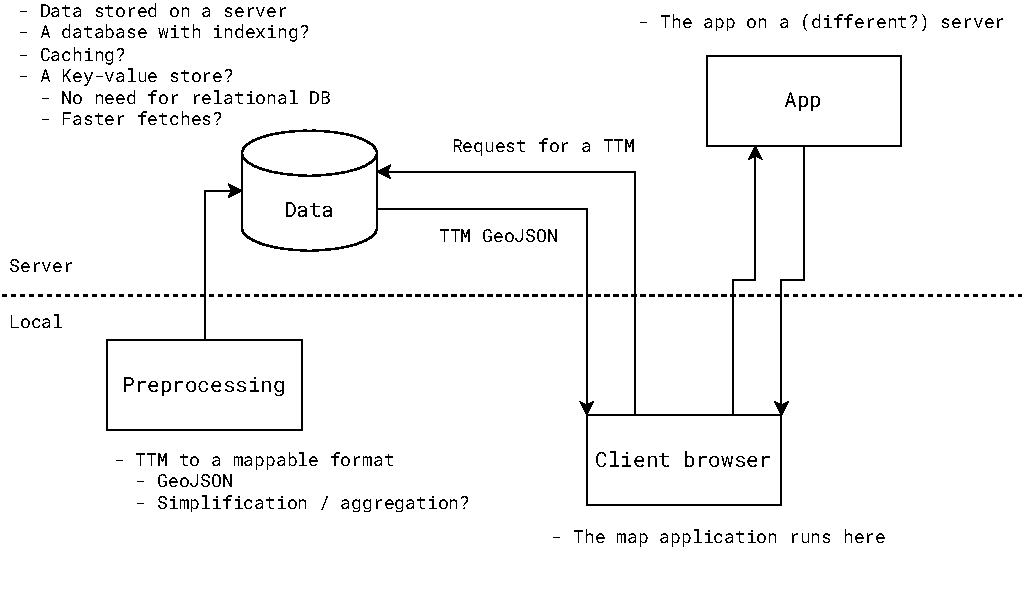
\includegraphics[width=1\textwidth]{visual/architechture}
	\caption{Architecture}
	\label{fig:architechture}
\end{figure}

% I see the methods necessary to implement the visualisation belonging to two themes:
% Methods for figuring out how the map should be
% and methods for actually making the map be that way.

% For figuring out what the map should be like,
% I have (hopefully) at this point already formed some ideas from the background section.
% To complement those, and to keep the qualitative aspect of cartography relevant,
% interview(s) will be used alongside the development process.

% When developing the visualisation, the priority should be on the map application.
% However, the development must progress on all components as an iterative process,
% where producing a minimal working state should be the first goal.
% Something that, to some extent, works, makes discussion about the map possible,
% which in turn should keep development progressing towards the right direction.

% It should also be noted that the number of techical options for implementing the map is large.
% Questions such as which mapping library or UI framework to use,
% or how to preprocess the matrix data should be covered here too.
% Depending on the need and extent of comparisons between different technologies,
% some synthesis could be formed about that too.

\subsection{Survey design}
structure of the survey,
analysis of the survey data.
